
\section{Sparse Marker Selection}
To construct an effective sparse marker set, our method exploits the full set of 13 markers recorded in the reference database and evaluates each marker's contribution to the whole-hand motion. 
% need description of the ref database if not given in Section 4
In constrast to the exhaustive search proposed by Kang et al.~\shortcite{KanWheZor12}, our technique computes the markers directly using PCA.

We conduct PCA with the Cartesian positions of the markers relative to the root link. With 13 markers, this leads to a PCA of motion data with 39 dimensions. In general, PCA produces a covariance matrix and the eigenvectors of this matrix create a list of components ordered from most important to least important.  
%
Each component has 39 coefficients that describe the influence of each marker on that component.  By adding up the contribution of each marker to all of the components, we can rank-order the influence of the markers on the full-set of components.  Furthermore, from the eigenvalues, we are given the relative importance of each principle component with respect to each other.  We can use this importance as a weighting to bias the components.  Thus, by summing the weighted contribution of each marker to each of the components, our marker rank ordering can account for the described bias.

%The marker coeffients are weighted depending 
%on how much the current component contributes to the final PCA reconstruction
%of the database and then summed. Markers with the highest sums are selected to
%be the sparse marker set.

In our results we highlight sparse marker sets of three and six markers, as those form the range of what can be captured and post-processed reasonably well based on our experience. 
Given the number of markers desired for the sparse set, we select the set simply as the top markers based on the rank-ordering.  We experimented with two methods of producing this rank-ordering, one with the eigenvalues acting as a weighting bias and the second treating all of the top-$N$ principle components as equally important and simply ignoring the remaining components. Conservatively experimenting with $N$ to be between one fourth and three fourths of the full dimensionality, these two approaches produced similar results.   However, if we selected $N$ to be the value of the full dimensionality, we did see reduced quality solutions.  In practice, we employ the eigenvalue weighted ranking for all results showcased in this paper.  

A nice feature of selecting the marker set in this fashion is that the rank-ordering simply adds subsequent markers from smaller sets to produce the larger sets. Thus, the described priority ranking reveals which are the definitively \emph{most} influential markers regardless of the
size of the sparse marker set. And so, in practice, adding more markers for higher quality recordings does not require a complete change of markers, only the addition of the desired number of markers to the ones employed in the lower quality recording.

%upon the respective marker's contribution to the PCA 
%reconstruction of the reference database.

\begin{figure*}[ht]
  \centering
  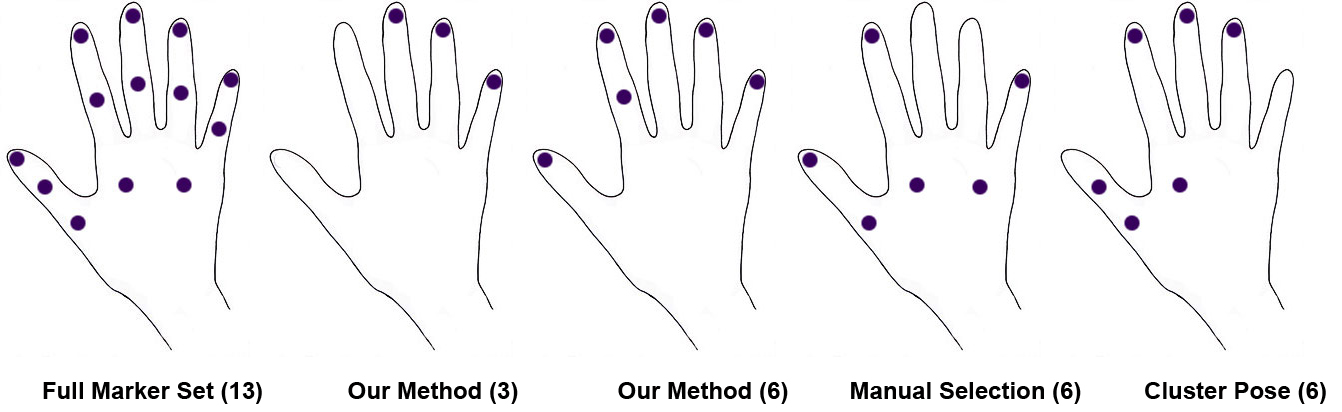
\includegraphics[trim = 0mm 0mm 0mm 0mm,
width=\textwidth]{images/marker_sets.jpg} %width=2.5in
  \caption{The tested marker sets.}
  \label{fig:marker_sets}
\end{figure*}




